\chapter{Related Work}\label{chapter:relatedWork}

\section{Scene Recognition Problem}\label{section:sceneRecognitionProblem}

Scene recognition is a problem that received a lot of attention from many researchers and engineers in the last few years. Even if approaches for several sensors were developed, the most popular is visual scene recognition based on images from a camera.\par
This section presents some of the most popular approaches for visual scene recognition based on traditional methods and machine learning.

\subsection{Local Image Descriptors}\label{section:localImageDescriptors}

This technique aims to find, describe and compare significant features from the images. Each image is processed in two phases: detection and description. Since both stages can be solved independently, a large number of various approaches for each phase have been developed.\par
The detection phase aims to detect all essential features in a given image, such as edges, corners, significant points, or objects. The feature detection algorithms generate pixel coordinates of each feature, usually with an occupied area. An example of the detected features in an image is shown in Figure \ref{fig:featuresDetection}. There are many different approaches to this problem, like FAST \parencite{FAST}, Laplacian of Gaussian \parencite{LaplacianOfGaussian}, SUSAN \parencite{SUSAN}, and many more, detecting different kinds of features.\par

\begin{figure}[htpb]
    \centering
    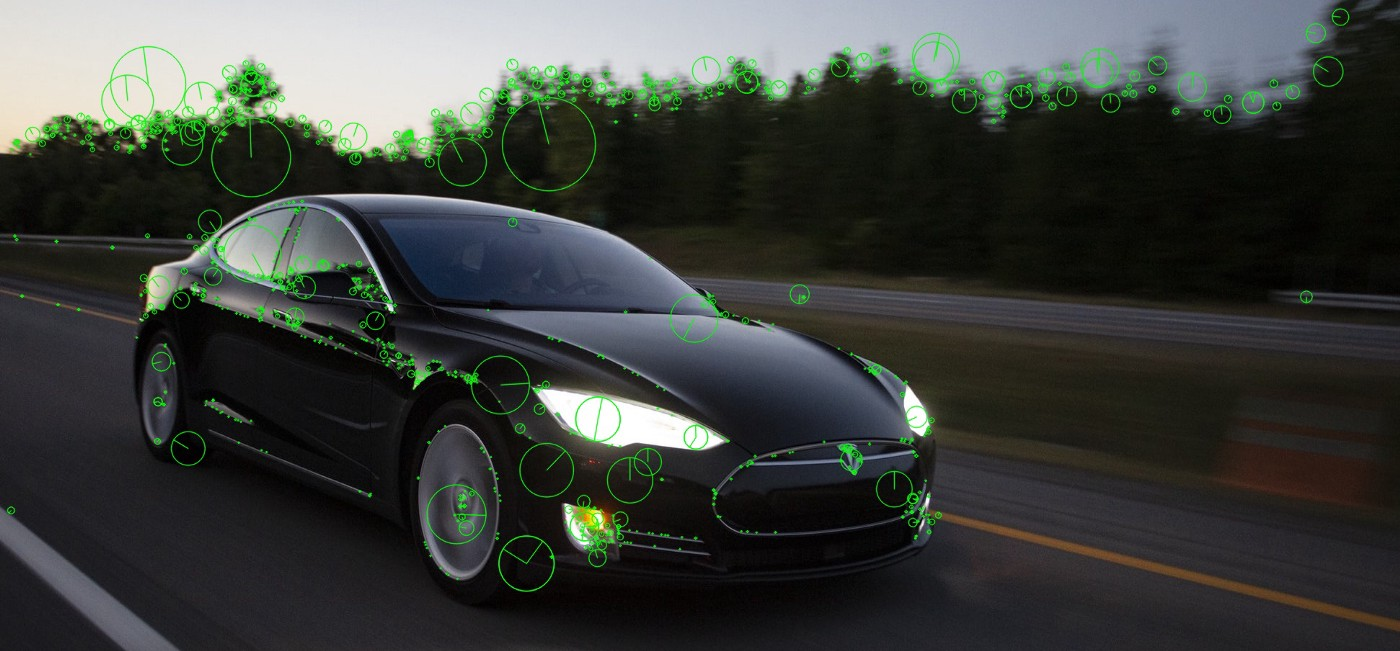
\includegraphics[width=0.8\textwidth]{featuresdet.jpeg}
    \caption{Example of detected features in the image. \cite{featuresImg}} \label{fig:featuresDetection}
\end{figure}

The goal of the description phase is to provide a summary of the image information around each feature. The feature is represented as its position in the image, and the output is defined as an N-dimensional vector. A good feature descriptor should fulfill three following rules: Repeatability, Distinctiveness, and Efficiency. The repeatability means that the feature descriptor is robust and invariant to the image's translation, rotation, or illumination changes. Distinctiveness represents the ability to distinguish between two close features. Finally, due to real-time processing, which is increasingly applied nowadays, efficiency also plays an important role. Among popular approaches to solve this problem can be included SURF \parencite{SURF}, GLOH \parencite{GLOH}, BRIEF \parencite{BRIEF}, and many more.\par
Using these two stages, the set of local image descriptors
$$
    \mathbf{X} = [\mathbf{x}_0, \mathbf{x}_1, \dots, \mathbf{x}_{n-1}]^T
$$
is extracted, in which $\textbf{x}_i \in \mathbb{R}^k$. However, each image can contain hundreds of individual features, which can be impractical in real-time processing and requires a huge amount of memory. To lower the dimensions of the local descriptors vector, different techniques like bag-of-visual-words \parencite{BagOfVisualWords1}\parencite{BagOfVisualWords2}, VLAD \parencite{VLAD}, or Fisher kernel \parencite{FisherKernel} may be applied to aggregate the vector $\mathbb{X}$ into a more compact single vector. Finally, these vectors are compared to decide if two images represent the same place. The precise comparison technique depends on the techniques used in the description phase and for the final descriptors' vector compression.

\subsection{Global Image Descriptors}\label{section:globalImageDescriptors}

This technique works similarly to the previous one, with one big difference. In this approach, the detection phase is wholly omitted, and the whole image is considered as only one feature. Therefore, the feature description algorithms must be modified to suitably describe large and diverse features. Some alternations of the algorithms provided in the last part might be WI\_SURF \parencite{WiSurf} or BRIEF-GIST \parencite{BRIEFGIST}.

\subsection{Neural Networks Based Approaches}\label{section:neuralNetworksBasedApproaches}

Convolutional neural networks achieve outstanding performance on several recognition or classification tasks, including a solution to scene recognition problems \parencite{CNNSceneRecognition1} \parencite{CNNSceneRecognition2}. The basic idea behind this approach is similar to the previously presented technique. In the first step, the global feature descriptor is extracted from the image and afterward compared with the other extracted feature vectors. However, unlike the previously presented technique, this approach uses machine learning instead of classical techniques to perform these two tasks.\par
According to the studies \cite{fischer2014descriptor}\cite{Imagenet}, the features extracted from images using convolutional neural networks significantly outperform the features extracted by classical algorithms like SIFT. There are many different kinds of convolutional neural networks used for these purposes. From the most popular ones, we can mention VGGNet \parencite{VggNet} or GoogleNet \parencite{GoogleNet}.

\section{OpenRatSLAM}\label{section:ratSlamRW}

OpenRatSLAM is an open source version of the RatSLAM approach implemented in ROS, see section \ref{section:ROS}. The system consists of the three most crucial components: Local view match, pose cell network, and experience map. Furthermore, the system contains one additional node, visual odometry, that can be optionally used to replace the odometry sensor with visual input. The way how these four parts communicate is presented in the picture \ref{fig:ratSlamCommunication}.\par

\begin{figure}[htpb]
    \centering
    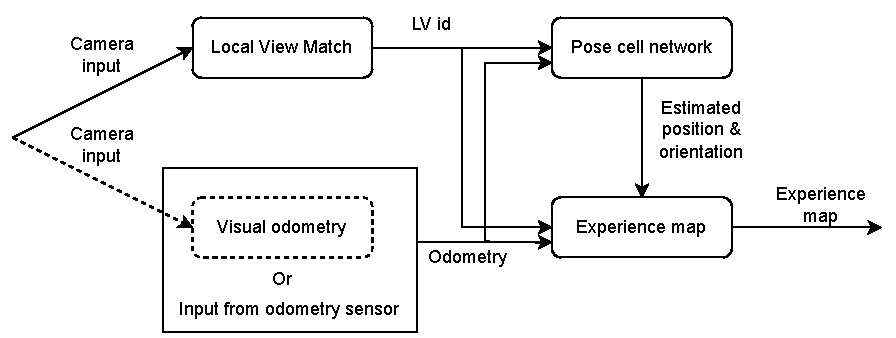
\includegraphics[width=0.8\textwidth]{ratSlamCoomunication.pdf}
    \caption{Nodes communication structure in the OpenRatSLAM} \label{fig:ratSlamCommunication}
\end{figure}

This section briefly introduces how each part of the RatSLAM works. For the detailed description, see \cite{RatSLAM} \cite{OpenRatSLAM}.

\subsection{Local View Match}\label{section:lvMatchROS}

This node receives an image from the camera and returns the id of the matched scene or a new id if no match is found. Firstly, the received image is converted into a local view template, represented as a strongly compressed grayscale image\footnote{In the experiments were used images with 60x10 px}. Before the conversion, global and local normalization steps are performed to lower light condition errors. After the normalization, the image is suitably compressed and converted to a grayscale image.\par
The generated template is compared with all the previously stored templates by calculating the sum of absolute differences. If the best result is below the chosen threshold, the id of the most similar scene is returned. If the best result is above the threshold, the scenes are estimated as different, and the current view template is stored with a new id, which will be returned.

\subsection{Visual Odometry}\label{section:visOdom}

This node's usage is necessary only when there is no odometry input from the sensors. This node aims to generate odometry data from camera input and thus replace the odometry sensor. The translational and rotational speed is calculated from changes in two regions of interest chosen in the incoming images. See \cite{RatSLAMExp2} for more details.

\subsection{Pose Cell Network}\label{section:poseCellsNet}

A pose cell network is a 3D structure of cells structured in a grid. Every cell represents a combination of the robot's position on $x$ and $y$ axes and orientation on the $z$ axe. The grid is also cyclic, meaning that the right-most cells are neighbors with the left-most cells or that the cells at the bottom are neighbors of the cells at the top of the grid. Each cell has an activity level, expressed by a real number between 0 and 1, where one means high activity and zero means no activity. Together with the grid of the pose cells, there exists a set of local view cells. The cells in this set arise during the program run, and every local view cell is connected with precisely one pose cell in the grid network. The network is visualized in Figure \ref{fig:ratSlam}\par

\begin{figure}[htpb]
    \centering
    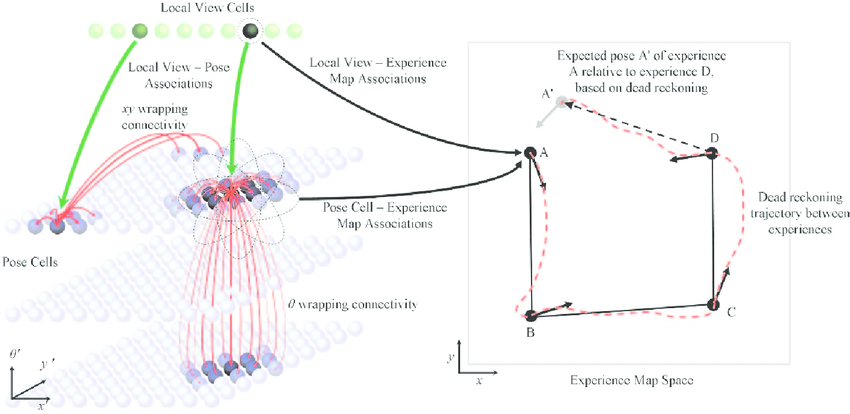
\includegraphics[width=0.8\textwidth]{GridNet.png}
    \caption{The OpenRatSLAM system structure. \cite{RatSLAMExp3}} \label{fig:ratSlam}
\end{figure}

During the algorithm run, there are usually more active pose cells. The bunch of active neighboring cells is called an activity packet. The final pose of the robot is estimated as the centroid of the activity packet. In the ideal situation, the grid contains only a single activity packet. However, several distinct activity packets could arise due to errors or inaccuracies in the sensors' data or LV match. In this case, the final pose is calculated as a centroid of the packet with the highest activity level.\par
Every time the Local view match node publishes an entirely new LV id, a new LV cell is created, connected with the pose cell representing the estimated current robot's position, and activated. When a known id is published, the corresponding local view cell is activated. There is always exactly one active local view cell.\par
The network's activity is updated in several steps: visual association, path integration, and normalization. At the beginning of the update step, the activity level of the cells around the pose cell, connected with the activated local view cell, is excited or inhibited according to the normal distribution. The path integration process projects the activity of the pose cells into cells near the currently activated ones. If the robot is translating, the activity is shifted in the $xy$ plane; if the robot is rotating activity is shifted in the $z$ direction. Under translation, the direction of movement of activity is dependent upon the cell's position in the $z$ direction. The magnitude of the movement in the $xy$ plane and $z$ axis depends on the translational and rotational velocity.\cite{RatSLAM} The total activation level of the network is designed to be 1. Therefore, after performing the visual association and path integration phases, the activilty level of all the cells is normalized.

\subsection{Experience Map}\label{section:expMap}

The experience map produces a graph-like map based on the network's activity, which is the final output of the algorithm. The map nodes, called experiences, correspond to the individual positions estimated by the pose cells together with the estimated local views. The experiences are connected with the links containing information about the relative pose, estimated from the odometry data and updated over time.\par
The map contains a map relaxation technique, which merges or removes experiences based on their similarities and accumulated errors. This technique makes the map more compact and the whole algorithm more robust against measures or estimation errors.
